\apendice{Especificación de diseño}

\section{Introducción}

\section{Diseño de datos}

\section{Diseño procedimental}

\section{Diseño arquitectónico}

\section{Diseño de interfaces}

Inicialmente se realizaron una serie de prototipos básicos en los que se plasmaron las principales funcionalidades de la aplicación, sin prestar especial atención a los aspectos estéticos de la misma. Para ello se usó la herramienta de prototipado Pencil, ya que permite incorporar elementos propios de la guía de estilos que se ha seguido para el diseño de las interfaces de usuario: \textit{Material Design}. 

\begin{figure}
	\centering
	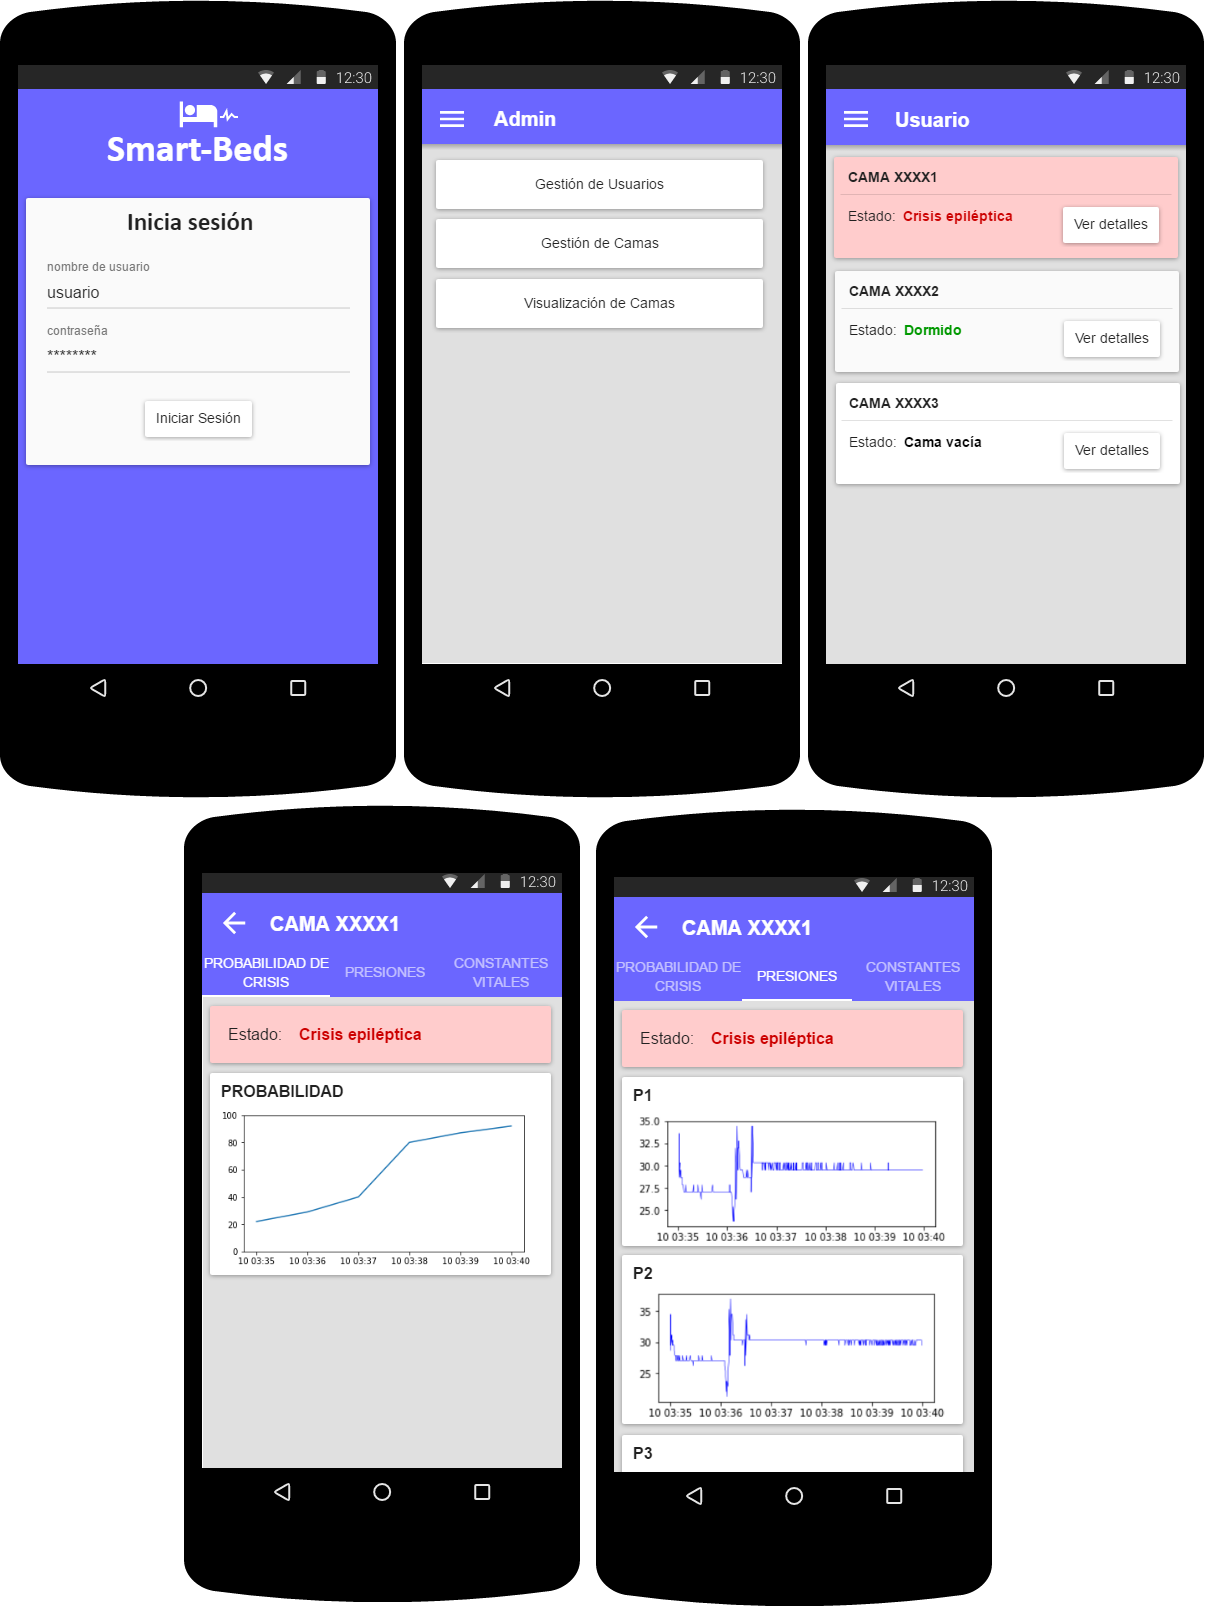
\includegraphics[width=1\textwidth]{../img/prototipos.png}
	\caption{Prototipos iniciales de las pantallas de: login, administración, visualización de camas y visualización de datos.}
	\label{fig:prototipos}
\end{figure}
